% This file was created with tikzplotlib v0.9.17.
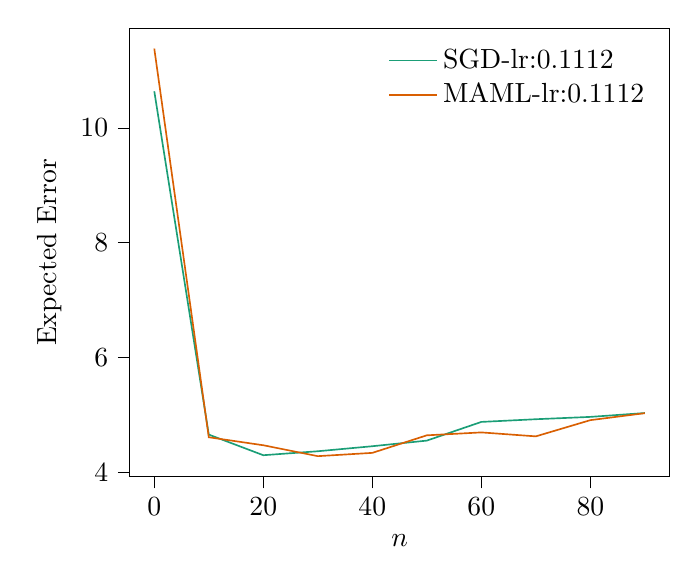
\begin{tikzpicture}

\definecolor{color0}{rgb}{0.105882352941176,0.619607843137255,0.466666666666667}
\definecolor{color1}{rgb}{0.850980392156863,0.372549019607843,0.00784313725490196}

\begin{axis}[
legend cell align={left},
legend style={fill opacity=0.8, draw opacity=1, text opacity=1, draw=none},
tick align=outside,
tick pos=left,
x grid style={white!69.0196078431373!black},
xlabel={\(\displaystyle n\)},
xmin=-4.5, xmax=94.5,
xtick style={color=black},
y grid style={white!69.0196078431373!black},
ylabel={Expected Error},
ymin=3.9298241829897, ymax=11.7350523410278,
ytick style={color=black}
]
\addplot [semithick, color0]
table {%
0 10.6365612078451
10 4.66023417360797
20 4.30094061296796
30 4.37007585035614
40 4.45753725888786
50 4.55538495020387
60 4.88075665283292
70 4.92763230488235
80 4.96830381710264
90 5.03555396617233
};
\addlegendentry{SGD-lr:0.1112}
\addplot [semithick, color1]
table {%
0 11.3802692429352
10 4.61378737208703
20 4.47445162244516
30 4.28460728108234
40 4.34194818882938
50 4.64735376126415
60 4.69814037795148
70 4.62934797023313
80 4.91150236515115
90 5.03290479450539
};
\addlegendentry{MAML-lr:0.1112}
\end{axis}

\end{tikzpicture}
